\section{多质点体系的引力作用}\label{sec:04.07}

我们知道,牛顿的万有引力定律式\eqref{eqn:04.03.04} 
\begin{equation}\label{eqn:04.07.01}
	F = \frac { G m _ { 1 } m _ { 2 } } { r ^ { 2 } }  
\end{equation}
是对两个质点而言的。牛顿在发展引力理论过程中,重要的一步
是把月亮运动和落体运动统一起来。在这个分析中,一个关键的
问题是牛顿认为地球表面落体运动的加速度可以写为
\begin{equation}\label{eqn:04.07.02}
	g = \frac { G M _ \text{地} } { R ^ { 2 } } 
\end{equation}
其中$ R $是地球半径。其实式\eqref{eqn:04.07.02}是直接从式\eqref{eqn:04.07.01}得来的。
这里有一个很大的疑问,为什么能把地球和落体间的距离看为$ R $?
如果说在讨论月亮运动时,把地球和月亮看作质点是一个足够好
的近似,那么讨论落体运动时,把地球看作质点显然是不合理的
\begin{wrapfigure}[11]{r}{17em}
	\centering
	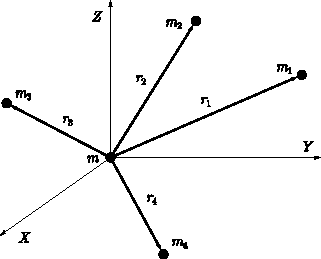
\includegraphics{figure/fig04.09}
	\caption{多质点体系的引力}
	\label{fig:04.09}
\end{wrapfigure}
牛顿一开始就意识到这一点,他感到不加证明地取地球和落体间距离
为R,从理论上来说是有欠缺的。后来,他给出了严格的证明。为了
研究这个问题,我们必须来讨论一下多质点体系的引力问题。

现在我们先来讨论一种简单情况。如图\ref{fig:04.09}~
% 145.jpg
所示,在原点有一质量为m的质点,空间分布着质量分别为$ m _ { 1 } $,
$ m _ { 2 }   $,$  m _ { 3 }   $,$ \cdots $,$ m _ { i } $的若干个质点,它们的位置矢径分别为$  r _ { 1 }   $,$  r _ { 2 }   $,$ 
r _ { 3 }   $,$ \cdots $, $ r _ { i } $。为了求质点$ m $所受到的引力,必须把式\eqref{eqn:04.07.01}作
些推广。根据式\eqref{eqn:04.07.01}可知:
{\setlength{\mathindent}{2em}
\begin{equation}\label{eqn:04.07.03}
	\begin{aligned}
\mbox{}&\text{第一个质点对}\,m\,\text{的引力为} \quad
 & \vec{F} _ { 1 } = \frac { G m m _ { 1 } } { r _ 1 ^ { 2 } } \cdot \frac { \vec{r} _ { 1 } } { r _ { 1 } }  \\  
\mbox{}&\text{第二个质点对}\,m\,\text{的引力为} \quad
& \vec{F} _ { 2 } = \frac { G m m _ { 2 } } { r _ 2 ^ { 2 } } \cdot \frac { \vec{r} _ { 2 } } { r _ { 2 } }  \\  
\mbox{}&\cdots \cdots \cdots \cdots \\
\mbox{}&\text{第}\;i\,\text{个质点对}\,m\,\text{的引力为} \quad
& \vec{F} _ { i } = \frac { G m m _ { i } } { r _ i ^ { 2 } } \cdot \frac { \vec{r} _ { i } } { r _ { i } }  \\  
\end{aligned}
\end{equation}}
式中$ \frac { \vec{r} _ { i } } { r _ { i } } $表示第$ i $个质点对$ m $的引力的方向。因此,可以自然地认
为,$ m $所受到的总力为
\begin{equation}\label{eqn:04.07.04}
	\begin{aligned}
\vec{F} &= \erratanote{\ensuremath{\vec{F}}}{原文作“\ensuremath{\vec{F}_1}”。(\ref{sec:04.07}节)} _ { 1 } + \vec{F} _ { 2 } + \cdots + \vec{F} _ { i }  \\
&= \sum _ i  { \frac { G m m _ { i } } { r _ { i } ^ 2 }  \cdot \frac { \vec{r} _ { i } } { r _ { i } } } 
\end{aligned}
\end{equation}

应当指出,这个推广中暗含了一个新观点。式\eqref{eqn:04.07.04}并不
全同于\eqref{eqn:04.07.01}所包含的物理内容,因为式\eqref{eqn:04.07.01}只说了两个质
点间的引力作用,而式\eqref{eqn:04.07.04}的写法,在本质上是认为两质点之
间的引力作用只与这两质点有关,而与第三者、第四者等等是否
存在毫无关系,可以不加顾及。这个新的物理内容是引力的一个
重要性质,我们称之为引力的线性迭加性。并不是所有的力都有
这种性质,譬如,强相互作用就没有这种性质。

做了上述推广,就可以来讨论牛顿所遇到的问题了。

考虑一密度均匀的球壳(图4·10),它的厚度t比它的半径r
小得多。我们要求出它对球壳外一个质量为$ m $的质点$ P $的引力。

可以把球壳看成许多小块的集合,每个小块在P点上都有作
